\documentclass{article}
\usepackage[margin=1in]{geometry} % Set margins to 1 inch
\usepackage[colorlinks=true, urlcolor=blue, linkcolor=red]{hyperref}
\usepackage{graphicx}
\usepackage{listings}
\usepackage{xcolor}
\usepackage{dirtree}

\definecolor{codegreen}{rgb}{0,0.6,0}
\definecolor{codegray}{rgb}{0.5,0.5,0.5}
\definecolor{codepurple}{rgb}{0.58,0,0.82}
\definecolor{backcolour}{rgb}{0.95,0.95,0.92}

\lstdefinestyle{mystyle}{
    backgroundcolor=\color{backcolour},   
    commentstyle=\color{codegreen},
    keywordstyle=\color{magenta},
    numberstyle=\tiny\color{codegray},
    stringstyle=\color{codepurple},
    basicstyle=\ttfamily\footnotesize,
    breakatwhitespace=false,         
    breaklines=true,                 
    captionpos=b,                    
    keepspaces=true,                 
    numbers=left,                    
    numbersep=5pt,                  
    showspaces=false,                
    showstringspaces=false,
    showtabs=false,                  
    tabsize=2
}

\lstset{style=mystyle}

\begin{document}

\title{\textbf{Creating Your First ROS2 Application}}
\author{Ameer Hamzah (Robotics Engineer)}
\date{Mar 4, 2024}
\maketitle

\section{Creating your first ROS Application}
Up until now, we have seen the paradigm behind a ROS project; however, we have still no clue on how to start a project from scrap.
The most attentious readers may have figured out (from what we said about the source command in the first lecture) that ROS works with different workspaces which contain everything you need to run your code, and they would be right.
In fact, a ROS project is exactly another workspace to source below the ros2 dependencies, once you do that, running your ROS project is no different from running a new TurtleSim node.

We will now see how we can build workspace and packages to organize our code, and then, how to write a simple publisher function.
At the end of this part, you should be able to instruct your turtle to move in a particular way just by running your written code.

\vspace{10pt} 
Let's get started!

\vspace{12pt} 
\textbf{NOTE: Make sure that ROS2 Humble is installed before following the steps given below.}
\subsection{Installing and Using Colcon to Build ROS2 Packages}
In this part, we will be using the tool colcon to build our first ROS package.
Let's install it before.
If you're using Ubuntu, just run: 
\begin{verbatim}
    sudo apt install python3-colcon-common-extensions 
\end{verbatim}
With that done, we are ready to use colcon.
\subsection{Creating a Workspace for Your First Project}
Let's start by creating a single folder \textit{ros2} for your workspace. Then create a folder named \textit{src} in it.
You can use the following command to do that in one step:
\begin{verbatim}
    mkdir -p ros2/src
\end{verbatim}
Move to your \textit{src} folder using \texttt{cd ros2/src} and create a new ros2 package by running:
\begin{verbatim}
    ros2 pkg create --build-type ament_python --node-name my_node my_package 
\end{verbatim}
Here, we are also creating a simple node as an example. If you only want to create a package, you can do it by running:
\begin{verbatim}
    ros2 pkg create --build-type ament_python [package_name]
\end{verbatim}
In terminal, move to your workspace using \texttt{cd ..} from your \textit{src} folder and run:
\begin{verbatim}
    colcon build
\end{verbatim}
This will build your workspace. Make sure that you have sourced the ros2 environment before running build command using:
 \begin{verbatim}
    source /opt/ros/humble/setup.bash
\end{verbatim}
You have sucessfully built your package now. Let's source the newly built workspace.
\begin{verbatim}
    source install/local_setup.bash
\end{verbatim}
Now, let's run our node.
\begin{verbatim}
    ros2 run my_package my_node
\end{verbatim}
You should get this output in the terminal.
\begin{figure}[h]
    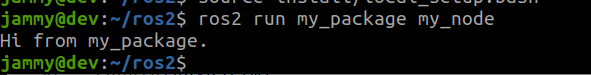
\includegraphics[width=12cm]{./data/images/pic0.png}
    \centering
    \caption{Output of Node}
\end{figure}    

Your \textit{ros2} workspace folder is comprised of this content now:
\vspace{12pt}
\dirtree{%
.1 ros2.
.2 build.
.2 install.
.2 log.
.2 src.
.3 my\textunderscore package.
}
\vspace{12pt}
You will do most of your work in \textit{src} folder. So, let's break down this folder to understand what's inside it.
\vspace{12pt}
\dirtree{%
.1 src.
.2 my\textunderscore package.
.3 my\textunderscore package.
.4 \textunderscore\textunderscore init.py\textunderscore\textunderscore.
.4 my\textunderscore node.py.
.3 resource.
.3 test.
.3 package.xml.
.3 setup.cfg.
.3 setup.py.
}
\vspace{12pt}
Let's create a new node now. Go inside my\textunderscore package folder in my\textunderscore package and create a new file \texttt{test.py}.
my\textunderscore package folder has now this content after the creation of new file.
\vspace{12pt}
\dirtree{%
.1 my\textunderscore package.
.2 my\textunderscore package.
.3 \textunderscore\textunderscore init.py\textunderscore\textunderscore.
.3 my\textunderscore node.py.
.3 test.py.
}
\vspace{12pt}
Open \texttt{test.py} file and write the following code inside it.
\pagebreak
\lstinputlisting[language=Python, caption={Script of Test Node}]{./data/snippets/test.py}
Save it and now we have to add entry points in the \texttt{setup.py} file so that we can get executable of this new python node.
\lstinputlisting[language=Python, caption={Adding entry point for test node}]{./data/snippets/entrypoints.py}
Let's now build it after moving to workspace folder i-e \textit{ros2} in this case
\begin{verbatim}
    colcon build
\end{verbatim}
This will build your workspace. Make sure that you have sourced the ros2 environment before running build command using:
 \begin{verbatim}
    source /opt/ros/humble/setup.bash
\end{verbatim}
You have sucessfully built your package now. Let's source the newly built workspace.
\begin{verbatim}
    source install/local_setup.bash
\end{verbatim}
Now, let's run our node.
\begin{verbatim}
    ros2 run my_package test.py
\end{verbatim}
You should get this output in the terminal.
\begin{figure}[h]
    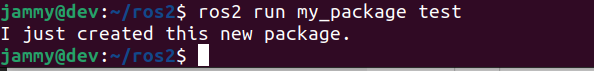
\includegraphics[width=12cm]{./data/images/pic1.png}
    \centering
    \caption{Output of Test Node}
\end{figure}
\subsection{Creating a Launch File}
To start multiple nodes at once, we use launch files. Here is an example of launch file written in python.
In order to create a launch file, go inside the \texttt{my\textunderscore package} folder and create a folder with name \textit{launch}. Inside this folder, create a new python file with name \texttt{simple\textunderscore launch.py}
\lstinputlisting[language=Python, caption={Launch File Script}]{./data/snippets/simple_launch.py}
To make this launch file work, you'll have to go to \texttt{setup.py} and modify the code as given below. Only add lines which are HASHED in the code below.
\lstinputlisting[language=Python, caption={Setup.py Modification for Launch File}]{./data/snippets/import.py}
Get back to your workspace and run \texttt{colcon build}. Source newly built workspace and run:
\begin{verbatim}
    ros2 launch my_package simple_launch.py
\end{verbatim}
Both nodes should run smoothly and you can check the data of both nodes by going to log folder as mentioned in the message that you will get once you run the launch file.  

\begin{thebibliography}{3}
    \bibitem{author1}
    Open Robotics. ``\textit{ROS2 Humble Official Documentation}''

    \bibitem{author3}
    Ameer Hamzah ``\textit{Proceedings of Aerial Robotics Lab, SINES, NUST, Pakistan}''. 2024.


\end{thebibliography}

\end{document}